\section{线性方程组，向量，矩阵}

\subsection{从方程组到矩阵}

先看一个三元方程组：
\[
\begin{cases}
x_1+2x_2+x_3=3,\\
2x_1+5x_2-x_3=-4,\\
3x_1-2x_2-x_3=5.
\end{cases}
\]
消元时写不写 \(x_1,x_2,x_3\) 不影响计算，真正起作用的只有系数和右边的常数。把系数按原来的位置排成数表，最后一列写常数项，得到
\[
\left(\begin{array}{ccc|c}
1 & 2 & 1 & 3\\
2 & 5 & -1 & -4\\
3 & -2 & -1 & 5
\end{array}\right).
\]
这张表叫\textbf{增广矩阵}。去掉最后一列，剩下的 \(3\times 3\) 数表叫\textbf{系数矩阵}。第 \(i\) 行第 \(j\) 列的元素 \(a_{ij}\) 是第 \(i\) 个方程中 \(x_j\) 的系数；最后一列不是任何未知数的系数，只放等号右边的数。

解方程时只允许做三件事：交换两个方程；把一个方程乘上非零常数；把一个方程的 \(k\) 倍加到另一个方程上。这三件事都不改变解集。搬到矩阵上，就是三种\textbf{初等行变换}：
\begin{enumerate}
\item 交换两行；
\item 用非零数 \(k\) 乘某一行；
\item 把第 \(j\) 行的 \(k\) 倍加到第 \(i\) 行（\(i\ne j\)）。
\end{enumerate}
只对行做。列变换相当于给未知数重新编号，做下去得到的解不对应原来的未知数，所以解方程组时不用列变换。但列变换和行变换一样，不改变矩阵的秩。

为什么行变换不改变解集？每条新方程都是旧方程的线性组合，新方程组的解自然满足旧方程组。反过来，三种操作都能撤销：交换再交换就回去，乘 \(k\) 再乘 \(1/k\) 就回去，加 \(k\) 倍再减 \(k\) 倍就回去。所以旧解也满足新方程组。

行变换的目标是把矩阵化成\textbf{行阶梯形}：每个非零行从左往右第一个非零元素叫\textbf{主元}，主元的位置逐行右移；主元正下方的元素全是 \(0\)；零行排在最后。如果再进一步，把每个主元化成 \(1\)，并把主元所在列的其余元素都化成 \(0\)，得到的就是\textbf{行最简形}，解可以直接读出来。

用行变换解开头那个方程组：
\[
\left(\begin{array}{ccc|c}
1 & 2 & 1 & 3\\
2 & 5 & -1 & -4\\
3 & -2 & -1 & 5
\end{array}\right)
\xrightarrow{r_2-2r_1,\ r_3-3r_1}
\left(\begin{array}{ccc|c}
1 & 2 & 1 & 3\\
0 & 1 & -3 & -10\\
0 & -8 & -4 & -4
\end{array}\right),
\]
\[
\left(\begin{array}{ccc|c}
1 & 2 & 1 & 3\\
0 & 1 & -3 & -10\\
0 & -8 & -4 & -4
\end{array}\right)
\xrightarrow{r_3+8r_2}
\left(\begin{array}{ccc|c}
1 & 2 & 1 & 3\\
0 & 1 & -3 & -10\\
0 & 0 & -28 & -84
\end{array}\right)
\xrightarrow{r_3/(-28)}
\left(\begin{array}{ccc|c}
1 & 2 & 1 & 3\\
0 & 1 & -3 & -10\\
0 & 0 & 1 & 3
\end{array}\right).
\]

最后得到的矩阵，其阶梯结构可以用一张图看清：

\begin{center}
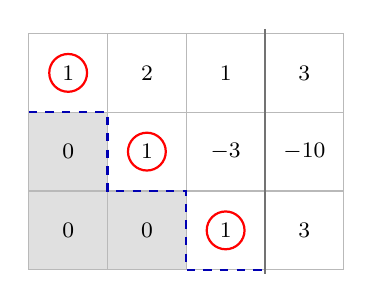
\begin{tikzpicture}[font=\footnotesize,scale=1.0]
% 阶梯下方的零元素
\fill[gray!24] (0,-1) rectangle (1,-2);
\fill[gray!24] (0,-2) rectangle (1,-3);
\fill[gray!24] (1,-2) rectangle (2,-3);
% 网格
\foreach \i in {1,2,3}{
  \foreach \j in {1,2,3,4}{
    \draw[gray!55] (\j-1,1-\i) rectangle ++(1,-1);
  }
}
% 元素
\node at (0.5,-0.5) {$1$}; \node at (1.5,-0.5) {$2$}; \node at (2.5,-0.5) {$1$}; \node at (3.5,-0.5) {$3$};
\node at (0.5,-1.5) {$0$}; \node at (1.5,-1.5) {$1$}; \node at (2.5,-1.5) {$-3$}; \node at (3.5,-1.5) {$-10$};
\node at (0.5,-2.5) {$0$}; \node at (1.5,-2.5) {$0$}; \node at (2.5,-2.5) {$1$}; \node at (3.5,-2.5) {$3$};
% 增广分隔线
\draw[black!55,thick] (3,0.06) -- (3,-3.06);
% 阶梯边界
\draw[blue!70!black,thick,dashed] (0,-1) -- (1,-1) -- (1,-2) -- (2,-2) -- (2,-3) -- (3,-3);
% 主元
\foreach \p in {(0.5,-0.5),(1.5,-1.5),(2.5,-2.5)}{
  \draw[red,thick] \p circle (0.24);
}
\end{tikzpicture}
\end{center}
\noindent{\small 红圈标出的是主元，它们的位置逐行右移。灰格里的元素必须为零，虚线就是阶梯的边界。最后一列是常数项，不参与选主元。}

接着回代。最后一行给出 \(x_3=3\)；代入第二行，\(x_2=-10+3x_3=-1\)；再代入第一行，\(x_1=3-2x_2-x_3=2\)。解为
\[
(x_1,x_2,x_3)=(2,-1,3).
\]
代回原方程组可以验算，三个等式都成立。如果继续化到行最简形，右端一列就是解，可以省掉回代。

化到行阶梯形后，解的情况只有三种：
\begin{enumerate}
\item 出现形如 \(0= d\)（\(d\ne 0\)）的矛盾行，无解；
\item 没有矛盾行，且主元个数等于未知数个数，解唯一；
\item 没有矛盾行，且主元个数小于未知数个数，有自由未知量，解有无穷多个。
\end{enumerate}
第三种情形里，自由未知量可以任取，每取一组值就得到一个解。

在计算机上做消元，还要多一步：选主元。先把绝对值最大的元素换到主元位置，再做除法，舍入误差会小很多。方程组的条件数 \(\kappa(A)\) 越大，输入的小扰动被放大得越厉害，解对舍入误差也越敏感。

\subsection{矩阵的运算}

\(m\times n\) 矩阵就是 \(m\) 行 \(n\) 列的数表，记作 \(A=(a_{ij})_{m\times n}\)。\(m=n\) 时叫方阵。

同型矩阵才能相加，规则是元素对应相加：\((A+B)_{ij}=a_{ij}+b_{ij}\)。数乘是每个元素都乘 \(k\)：\((kA)_{ij}=ka_{ij}\)。这两种运算都满足交换律、结合律和分配律。

矩阵乘法要复杂一些。先看形状：左矩阵的列数必须等于右矩阵的行数。设 \(A=(a_{ij})_{m\times s}\)，\(B=(b_{ij})_{s\times n}\)，则 \(C=AB\) 是 \(m\times n\) 矩阵，其元素为
\[
c_{ij}=\sum_{k=1}^{s}a_{ik}b_{kj}
=a_{i1}b_{1j}+a_{i2}b_{2j}+\cdots+a_{is}b_{sj}.
\]
也就是说，\(c_{ij}\) 是 \(A\) 的第 \(i\) 行与 \(B\) 的第 \(j\) 列对应相乘再相加。

\begin{center}
\begin{tikzpicture}[font=\footnotesize,scale=1.12]
% 矩阵 A
\fill[blue!18] (0,0.7) rectangle (2.7,1.4);
\foreach \i in {0,1,2}{
  \foreach \j in {0,1,2}{
    \draw[gray!55] (0.9*\j,0.7*\i) rectangle ++(0.9,0.7);
  }
}
\node at (0.45,1.05) {$a_{i1}$};
\node at (1.35,1.05) {$a_{i2}$};
\node at (2.25,1.05) {$\cdots$};
\node at (1.35,0.35) {$\vdots$};
\node at (1.35,1.75) {$\vdots$};
% 矩阵 B
\fill[red!15] (4.5,0) rectangle (5.4,2.1);
\foreach \i in {0,1,2}{
  \foreach \j in {0,1}{
    \draw[gray!55] (3.6+0.9*\j,0.7*\i) rectangle ++(0.9,0.7);
  }
}
\node at (4.95,1.75) {$b_{1j}$};
\node at (4.95,1.05) {$\vdots$};
\node at (4.95,0.35) {$b_{sj}$};
% 矩阵 C
\fill[green!18] (7.3,0.35) rectangle (8.2,1.05);
\foreach \i in {0,1}{
  \foreach \j in {0,1}{
    \draw[gray!55] (6.4+0.9*\j,0.35+0.7*\i) rectangle ++(0.9,0.7);
  }
}
\node at (7.75,0.7) {$c_{ij}$};
% 箭头
\draw[->,thick,gray] (2.78,1.05) -- (3.52,1.05);
\draw[->,thick,gray] (5.48,0.7) -- (6.32,0.7);
% 标题
\node[above] at (1.35,2.1) {$A$：\(m\times s\)};
\node[above] at (4.5,2.1) {$B$：\(s\times n\)};
\node[above] at (7.3,1.75) {$C=AB$：\(m\times n\)};
% 公式
\node at (4.1,-0.55) {$c_{ij}=a_{i1}b_{1j}+a_{i2}b_{2j}+\cdots+a_{is}b_{sj}$};
\end{tikzpicture}
\end{center}
\noindent{\small 蓝行与红列配对，得到绿格的 \(c_{ij}\)。三张表的尺寸必须首尾相接：\(A\) 的列数等于 \(B\) 的行数，结果的尺寸是 \(m\times n\)。}

这样定义是为了保证结合律，也让矩阵乘法对应线性变换的复合：先做 \(B\)，再做 \(A\)，就是 \(AB\)。换一个看法，\(AB\) 的第 \(j\) 列等于 \(A\) 乘 \(B\) 的第 \(j\) 列：
\[
AB=A(\boldsymbol b_1,\boldsymbol b_2,\ldots,\boldsymbol b_n)=(A\boldsymbol b_1,A\boldsymbol b_2,\ldots,A\boldsymbol b_n).
\]

\begin{center}
\[
A=\begin{pmatrix}1&2\\3&4\end{pmatrix},\qquad
B=\begin{pmatrix}2&0\\1&3\end{pmatrix}.
\]
\end{center}
计算得
\[
AB=\begin{pmatrix}4&6\\10&12\end{pmatrix},\qquad
BA=\begin{pmatrix}2&4\\10&14\end{pmatrix}.
\]
两个结果不一样，所以矩阵乘法一般不可交换。即使 \(A,B\) 都是方阵，\(AB\) 和 \(BA\) 也可能不相等。

乘法还有两个容易踩的坑。第一，消去律不成立：由 \(AB=AC\) 且 \(A\ne O\) 推不出 \(B=C\)。第二，有零因子：
\[
\begin{pmatrix}0&1\\0&0\end{pmatrix}
\begin{pmatrix}1&0\\0&0\end{pmatrix}
=\begin{pmatrix}0&0\\0&0\end{pmatrix},
\]
两个非零矩阵乘出了零矩阵。

转置把行和列互换，\((A^{\mathrm T})_{ij}=a_{ji}\)。转置与乘法相遇时要反序：
\[
(AB)^{\mathrm T}=B^{\mathrm T}A^{\mathrm T}.
\]
方阵的幂规定为 \(A^0=I_n\)，\(A^k=AA\cdots A\)（\(k\) 个）。因为 \(A\) 与自身可交换，\(A^kA^l=A^{k+l}\) 成立。但 \((AB)^k\ne A^kB^k\)，除非 \(AB=BA\)。同样，
\[
(A+B)^2=A^2+AB+BA+B^2,
\]
中间两项不能合并成 \(2AB\)。

\subsection{向量、线性组合与矩阵的秩}

\(n\) 个实数排成一列，叫 \(n\) 维列向量：
\[
\boldsymbol\alpha=\begin{pmatrix}a_1\\a_2\\\vdots\\a_n\end{pmatrix}.
\]
\(a_i\) 是第 \(i\) 个分量。两个同维向量相加是分量相加，数乘是每个分量乘同一个数。这两种运算的规律，和矩阵的加法、数乘一样。

内积把两个向量压成一个数：
\[
\boldsymbol\alpha^{\mathrm T}\boldsymbol\beta
=a_1b_1+a_2b_2+\cdots+a_nb_n.
\]
两个非零向量的内积为 \(0\)，就说它们垂直（正交）。向量长度是 \(\|\boldsymbol\alpha\|=\sqrt{\boldsymbol\alpha^{\mathrm T}\boldsymbol\alpha}\)，长度为 \(1\) 的叫单位向量。

给定向量 \(\boldsymbol\alpha_1,\ldots,\boldsymbol\alpha_n\) 和数 \(x_1,\ldots,x_n\)，和式
\[
x_1\boldsymbol\alpha_1+x_2\boldsymbol\alpha_2+\cdots+x_n\boldsymbol\alpha_n
\]
叫这组向量的一个\textbf{线性组合}，\(x_j\) 是组合系数。

矩阵乘向量，正好是列向量的线性组合。把 \(A\) 按列分块：
\[
A\boldsymbol x=(\boldsymbol\alpha_1,\boldsymbol\alpha_2,\ldots,\boldsymbol\alpha_n)
\begin{pmatrix}x_1\\x_2\\\vdots\\x_n\end{pmatrix}
=x_1\boldsymbol\alpha_1+x_2\boldsymbol\alpha_2+\cdots+x_n\boldsymbol\alpha_n.
\]
于是 \(A\boldsymbol x=\boldsymbol b\) 有解，等价于 \(\boldsymbol b\) 能由 \(A\) 的列向量线性表示，组合系数就是解。

\begin{center}
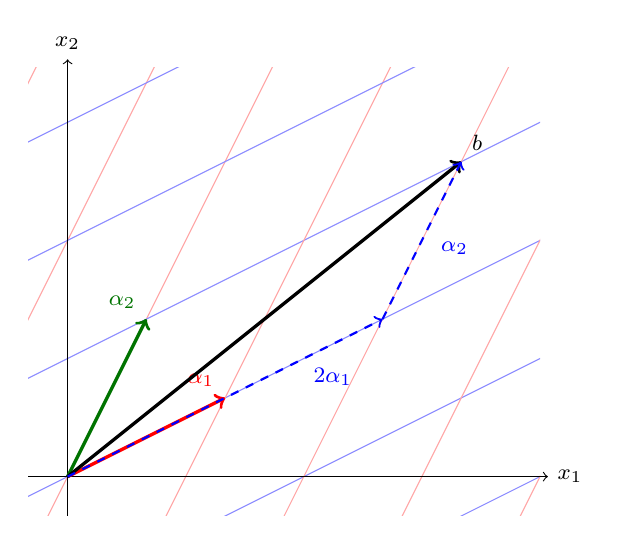
\begin{tikzpicture}[font=\footnotesize,scale=1.0]
\begin{scope}
\clip (-0.5,-0.5) rectangle (6.0,5.2);
\foreach \k in {-8,...,8}{
  \draw[blue!45] ({\k-12},{2*\k-6}) -- ({\k+12},{2*\k+6});
  \draw[red!35] ({2*\k-6},{\k-12}) -- ({2*\k+6},{\k+12});
}
\end{scope}
\draw[->] (-0.5,0) -- (6.1,0) node[right] {\(x_1\)};
\draw[->] (0,-0.5) -- (0,5.3) node[above] {\(x_2\)};
\draw[->,very thick,red] (0,0) -- (2,1) node[above left] {\(\boldsymbol\alpha_1\)};
\draw[->,very thick,green!45!black] (0,0) -- (1,2) node[above left] {\(\boldsymbol\alpha_2\)};
\draw[->,very thick,black] (0,0) -- (5,4) node[above right] {\(\boldsymbol b\)};
\draw[->,thick,blue,dashed] (0,0) -- (4,2);
\draw[->,thick,blue,dashed] (4,2) -- (5,4);
\node[blue,below right] at (3,1.5) {\(2\boldsymbol\alpha_1\)};
\node[blue,anchor=west] at (4.62,2.9) {\(\boldsymbol\alpha_2\)};
\end{tikzpicture}
\end{center}
\noindent{\small 两族平行线分别沿 \(\boldsymbol\alpha_1\) 和 \(\boldsymbol\alpha_2\) 的方向，它们的交点都是整数系数的组合。图中 \(\boldsymbol b=2\boldsymbol\alpha_1+\boldsymbol\alpha_2\)，所以方程 \(x_1\boldsymbol\alpha_1+x_2\boldsymbol\alpha_2=\boldsymbol b\) 有解 \((2,1)\)。系数允许取实数时，平面上的每个点都能到达；两个方向不共线，这就是原因。}

接下来给“独立方向的个数”一个名字。

\begin{mydef}{矩阵的秩}{rank}
把矩阵 \(A\) 用初等行变换化成行阶梯形，非零行的个数称为 \(A\) 的\textbf{秩}，记作 \(r(A)\) 或 \(\operatorname{rank}(A)\)。不同的化法得到的非零行数相同，所以秩由 \(A\) 本身决定。
\end{mydef}

设 \(A\) 是 \(m\times n\) 矩阵。同一个数有三种读法：
\begin{enumerate}
\item 行阶梯形中主元的个数，也就是独立方程的个数；
\item 列向量组中线性无关向量的最大个数，也就是列向量张成空间的维数；
\item 行向量组中线性无关向量的最大个数。行秩等于列秩，所以不必区分。
\end{enumerate}
秩还有两条基本性质：\(r(A)=r(A^{\mathrm T})\)，以及 \(r(A)\le\min(m,n)\)。

\begin{center}
\begin{tikzpicture}[font=\footnotesize,scale=0.9]
% 左：共线
\begin{scope}
\draw[->] (-1.6,0) -- (2.6,0) node[right] {\(x_1\)};
\draw[->] (0,-1.6) -- (0,2.6) node[above] {\(x_2\)};
\draw[gray!50] (-1.4,-1.4) -- (2.3,2.3);
\draw[->,very thick,red] (0,0) -- (1,1);
\draw[->,very thick,blue] (0,0) -- (2,2);
\draw[->,very thick,green!45!black] (0,0) -- (-1,-1);
\node[below right,red] at (0.55,0.55) {\(\boldsymbol\alpha_1\)};
\node[above left,blue] at (2,2) {\(\boldsymbol\alpha_2\)};
\node[below left,green!45!black] at (-1,-1) {\(\boldsymbol\alpha_3\)};
\node[align=center] at (0.4,-2.15) {张成一条直线\\\(r=1\)};
\end{scope}
% 右：不共线
\begin{scope}[xshift=6.4cm]
\draw[->] (-0.8,0) -- (3.5,0) node[right] {\(x_1\)};
\draw[->] (0,-1.2) -- (0,3.0) node[above] {\(x_2\)};
\fill[blue!15] (0,0) -- (1,1) -- (3,2) -- (2,1) -- cycle;
\draw[blue!45] (0,0) -- (1,1) -- (3,2) -- (2,1) -- cycle;
\draw[->,very thick,red] (0,0) -- (1,1);
\draw[->,very thick,blue] (0,0) -- (2,1);
\node[above left,red] at (1,1) {\(\boldsymbol\alpha_1\)};
\node[below right,blue] at (2,1) {\(\boldsymbol\alpha_2\)};
\node[align=center] at (1,-2.15) {张成整个平面\\\(r=2\)};
\end{scope}
\end{tikzpicture}
\end{center}
\noindent{\small 左图三个向量在同一条直线上，无论怎么组合都离不开这条直线，秩为 \(1\)。右图两个向量不共线，取不同的组合系数可以达到平面上的任意点，秩为 \(2\)。秩就是独立方向的个数。}

行变换不改变秩，也不改变列向量之间的线性关系：若某组系数使列向量的组合等于零，变换后同一组系数仍使它等于零。这就是行变换不改变解集的原因。

第 2 章会讨论向量组的极大线性无关组。那里会看到，\(r(A)\) 正是 \(A\) 的列向量组的极大无关组所含向量的个数。

\subsection{齐次方程组}

齐次方程组写成 \(A\boldsymbol x=\boldsymbol 0\)。它一定有解：\(\boldsymbol x=\boldsymbol 0\) 总是解，叫零解。问题是还有没有别的解。

设 \(A\) 是 \(m\times n\) 矩阵，\(r(A)=r\)。把 \(A\) 化成行最简形以后：
\begin{enumerate}
\item 主元所在的列对应\textbf{主变量}，共有 \(r\) 个；
\item 其余的列对应\textbf{自由变量}，共有 \(n-r\) 个。
\end{enumerate}
自由变量可以任取。每取一组值，主变量就被唯一确定。所以 \(r=n\) 时没有自由变量，只有零解；\(r<n\) 时有非零解，且有无穷多个。

能生成其余所有解的一组解，有专门的名字。
\begin{mydef}{基础解系}{fundamental-system}
齐次方程组 \(A\boldsymbol x=\boldsymbol 0\) 的一组解 \(\boldsymbol\xi_1,\ldots,\boldsymbol\xi_{n-r}\)，如果满足
\begin{enumerate}
\item 它们线性无关，即其中任何一个都不能由其余几个线性表示；
\item 方程组的每个解都能写成它们的线性组合，
\end{enumerate}
就称它们为一个\textbf{基础解系}。
\end{mydef}

具体做法：把自由变量依次取 \(1\)（其余自由变量取 \(0\)），解出主变量，得到 \(n-r\) 个解。它们就是基础解系。通解为
\[
\boldsymbol x=k_1\boldsymbol\xi_1+k_2\boldsymbol\xi_2+\cdots+k_{n-r}\boldsymbol\xi_{n-r},
\qquad k_1,\ldots,k_{n-r}\in\mathbb R.
\]

看一个例子。设
\[
A=\begin{pmatrix}1&1&1\\2&3&1\end{pmatrix}.
\]
化成行最简形：
\[
\begin{pmatrix}1&1&1\\2&3&1\end{pmatrix}
\xrightarrow{r_2-2r_1}
\begin{pmatrix}1&1&1\\0&1&-1\end{pmatrix}
\xrightarrow{r_1-r_2}
\begin{pmatrix}1&0&2\\0&1&-1\end{pmatrix}.
\]
这里 \(n=3\)，\(r=2\)，自由变量只有 \(x_3\)。方程化为
\[
x_1+2x_3=0,\qquad x_2-x_3=0.
\]
令 \(x_3=t\)，则 \(x_1=-2t\)，\(x_2=t\)，即
\[
\boldsymbol x=t\begin{pmatrix}-2\\1\\1\end{pmatrix}.
\]
基础解系只有一个向量 \(\boldsymbol\xi=(-2,1,1)^{\mathrm T}\)，通解是它的任意倍数。

从几何上看，齐次方程组的解集是 \(\mathbb R^n\) 中过原点的子空间，维数为 \(n-r\)。两个解相加、一个解乘上常数，仍然是解。

\begin{center}
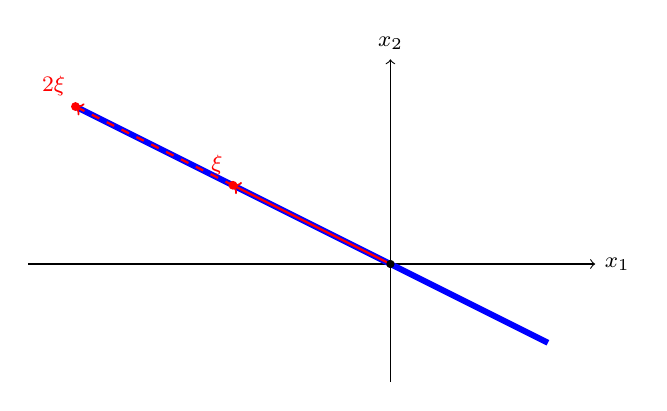
\begin{tikzpicture}[font=\footnotesize,scale=1.0]
\draw[->] (-4.6,0) -- (2.6,0) node[right] {\(x_1\)};
\draw[->] (0,-1.5) -- (0,2.6) node[above] {\(x_2\)};
\draw[blue,line width=2.2pt] (2,-1) -- (-4,2);
\draw[->,thick,red] (0,0) -- (-2,1) node[above left] {\(\boldsymbol\xi\)};
\draw[->,thick,red,dashed] (-2,1) -- (-4,2) node[above left] {\(2\boldsymbol\xi\)};
\fill[red] (-2,1) circle (1.6pt);
\fill[red] (-4,2) circle (1.6pt);
\fill (0,0) circle (1.5pt);
\end{tikzpicture}
\end{center}
\noindent{\small 两个未知数的齐次方程 \(x_1+2x_2=0\) 的解是一条过原点的直线。\(\boldsymbol\xi\) 是解，\(2\boldsymbol\xi\) 也是解；任取两个解相加，仍然落在直线上。解集对加法、数乘封闭，是一个一维子空间，维数正好是 \(n-r=2-1=1\)。}

\subsection{非齐次方程组与解的结构}

非齐次方程组写成 \(A\boldsymbol x=\boldsymbol b\)，\(\boldsymbol b\ne\boldsymbol 0\)。它可能无解，所以先判断相容性。

把增广矩阵 \((A\mid\boldsymbol b)\) 化成行阶梯形，比较两边的秩：
\begin{itemize}
\item 若 \(r(A)<r(A\mid\boldsymbol b)\)，最后一列出现主元，等价于某行变成 \(0=d\)（\(d\ne0\)），无解；
\item 若 \(r(A)=r(A\mid\boldsymbol b)=r\)，有解。此时 \(r=n\) 唯一解，\(r<n\) 有无穷多解。
\end{itemize}

有解时，解集的结构很整齐。

\begin{conclusion}{非齐次方程组解的结构}{nonhomogeneous-structure}
设 \(A\boldsymbol x=\boldsymbol b\) 有解，\(\boldsymbol\eta_0\) 是它的一个特解，\(\boldsymbol\xi_1,\ldots,\boldsymbol\xi_{n-r}\) 是对应齐次方程组 \(A\boldsymbol x=\boldsymbol 0\) 的基础解系。则 \(A\boldsymbol x=\boldsymbol b\) 的全部解为
\[
\boldsymbol x=\boldsymbol\eta_0+k_1\boldsymbol\xi_1+\cdots+k_{n-r}\boldsymbol\xi_{n-r},
\qquad k_i\in\mathbb R.
\]
\end{conclusion}

道理很短。若 \(\boldsymbol x\) 和 \(\boldsymbol\eta_0\) 都满足 \(A\boldsymbol x=\boldsymbol b\)，则
\[
A(\boldsymbol x-\boldsymbol\eta_0)=A\boldsymbol x-A\boldsymbol\eta_0=\boldsymbol b-\boldsymbol b=\boldsymbol 0,
\]
所以 \(\boldsymbol x-\boldsymbol\eta_0\) 是齐次方程组的解。反过来，\(\boldsymbol\eta_0\) 加上任一齐次解，仍然满足 \(A\boldsymbol x=\boldsymbol b\)。

把上一节的例子加上右端项：
\[
\left(\begin{array}{ccc|c}
1&1&1&2\\
2&3&1&3
\end{array}\right)
\xrightarrow{r_2-2r_1}
\left(\begin{array}{ccc|c}
1&1&1&2\\
0&1&-1&-1
\end{array}\right)
\xrightarrow{r_1-r_2}
\left(\begin{array}{ccc|c}
1&0&2&3\\
0&1&-1&-1
\end{array}\right).
\]
秩 \(r(A)=r(A\mid\boldsymbol b)=2<3\)，有无穷多解。方程化为
\[
x_1=3-2x_3,\qquad x_2=-1+x_3.
\]
令 \(x_3=t\)，得
\[
\boldsymbol x=\begin{pmatrix}3\\-1\\0\end{pmatrix}
+t\begin{pmatrix}-2\\1\\1\end{pmatrix}.
\]
其中 \((3,-1,0)^{\mathrm T}\) 是一个特解，\((-2,1,1)^{\mathrm T}\) 是齐次方程组的基础解系。通解就是“一个特解加齐次通解”。

\begin{center}
\begin{tikzpicture}[font=\footnotesize,scale=0.95]
\draw[->] (-3.6,0) -- (4.9,0) node[right] {\(x_1\)};
\draw[->] (0,-1.6) -- (0,3.6) node[above] {\(x_2\)};
\draw[gray,dashed,thick] (2,-1) -- (-3,1.5);
\draw[blue,thick] (4,-0.5) -- (-1,2);
\draw[->,thick,orange!80!black] (0,0) -- (1,1) node[below right] {\(\boldsymbol\eta_0\)};
\draw[->,very thick,red] (1,1) -- (-1,2) node[above left] {\(\boldsymbol\xi\)};
\fill[red] (1,1) circle (1.5pt);
\fill[red] (-1,2) circle (1.5pt);
\fill[red] (3,0) circle (1.5pt);
\node[blue,above right] at (2.55,0.32) {\(x_1+2x_2=3\)};
\end{tikzpicture}
\end{center}
\noindent{\small 以两个未知数为例。灰虚线是齐次方程的解，蓝线是非齐次方程的解。蓝线是灰线平移 \(\boldsymbol\eta_0\) 得到的，方向不变；线上的点都能写成 \(\boldsymbol\eta_0+t\boldsymbol\xi\)。所以非齐次解集不是子空间，它是齐次解子空间的一个平移。}

三种情形可以用一张表记住（以 \(n=2\)、两条直线为例）：
\begin{center}
\begin{tabular}{ccc}
\toprule
秩的关系 & 两条直线 & 解的情况 \\
\midrule
\(r(A)<r(A\mid\boldsymbol b)\) & 平行且不重合 & 无解 \\
\(r(A)=r(A\mid\boldsymbol b)=n\) & 交于一点 & 唯一解 \\
\(r(A)=r(A\mid\boldsymbol b)<n\) & 重合 & 无穷多解，\(n-r\) 个自由未知量 \\
\bottomrule
\end{tabular}
\end{center}

最后把两节合起来看。秩 \(r\) 是独立约束的个数，\(n-r\) 是自由度。齐次方程组的解集是 \(n-r\) 维子空间，非齐次方程组的解集是这个子空间平移一个特解。行变换、秩、解的结构，说的是同一件事。

\section{习题}

\subsection{本章速览}

\begin{itemize}
\item \textbf{初等行变换：}倍乘（乘非零数）、倍加、对换三种操作不改变方程组的解集。把矩阵化为行阶梯形后，非零行的行数就是矩阵的秩 \(r(A)\)。
\item \textbf{矩阵乘法：}左矩阵的列数必须等于右矩阵的行数，且 \(c_{ij}\) 是 \(A\) 的第 \(i\) 行与 \(B\) 的第 \(j\) 列的内积。矩阵乘法一般不可交换、不可消去；转置要反序：\((AB)^{\mathrm T}=B^{\mathrm T}A^{\mathrm T}\)。
\item \textbf{方阵的幂：}若 \(A=I+N\) 且 \(N^k=O\)，则 \(A^n=I+nN+\binom n2N^2+\cdots+N^n\)，因为 \(I\) 与 \(N\) 可交换，二项式展开成立。
\item \textbf{齐次方程组 \(A\boldsymbol x=\boldsymbol 0\)：}必有零解；只有零解 \(\iff r(A)=n\)；有非零解 \(\iff r(A)<n\)，此时基础解系含 \(n-r(A)\) 个向量，通解是它们的线性组合。
\item \textbf{非齐次方程组 \(A\boldsymbol x=\boldsymbol b\)：}有解 \(\iff r(A)=r(A\mid\boldsymbol b)\)。设此公共秩为 \(r\)：唯一解 \(\iff r=n\)；无穷多解 \(\iff r<n\)；通解 \(=\) 一个特解 \(+\) 对应齐次方程组的通解。
\item \textbf{含参讨论：}先做不含除法的行变换，把主元保留成含参数的因式；再按“主元为零”与“主元非零”分支讨论，切勿默认参数非零而约去。
\end{itemize}

\subsection{基础过关题}

\textbf{1.} 设
\[
A=\begin{pmatrix}1&2\\0&1\end{pmatrix},\qquad
B=\begin{pmatrix}1&0\\3&1\end{pmatrix}.
\]
求 \(AB\)，\(BA\)，\(A^2\)，并验证 \((AB)^{\mathrm T}=B^{\mathrm T}A^{\mathrm T}\)。

\ifshowsolutions%
\boxed{\textbf{解}}
\textbf{思路：}按“行乘列”逐元素计算；转置验证时先分别求 \(B^{\mathrm T}\)、\(A^{\mathrm T}\)，再按相反顺序相乘。

\[
AB=\begin{pmatrix}1\cdot1+2\cdot3&1\cdot0+2\cdot1\\0\cdot1+1\cdot3&0\cdot0+1\cdot1\end{pmatrix}
=\begin{pmatrix}7&2\\3&1\end{pmatrix},
\]
\[
BA=\begin{pmatrix}1\cdot1+0\cdot0&1\cdot2+0\cdot1\\3\cdot1+1\cdot0&3\cdot2+1\cdot1\end{pmatrix}
=\begin{pmatrix}1&2\\3&7\end{pmatrix},
\]
\[
A^2=\begin{pmatrix}1&2\\0&1\end{pmatrix}\begin{pmatrix}1&2\\0&1\end{pmatrix}
=\begin{pmatrix}1&4\\0&1\end{pmatrix}.
\]
又
\[
B^{\mathrm T}A^{\mathrm T}
=\begin{pmatrix}1&3\\0&1\end{pmatrix}\begin{pmatrix}1&0\\2&1\end{pmatrix}
=\begin{pmatrix}1+6&3\\0+2&1\end{pmatrix}
=\begin{pmatrix}7&3\\2&1\end{pmatrix}
=(AB)^{\mathrm T}.
\]
这里 \(AB\neq BA\)，说明矩阵乘法一般不满足交换律。

\boxed{\text{答案：}AB=\begin{pmatrix}7&2\\3&1\end{pmatrix},\quad BA=\begin{pmatrix}1&2\\3&7\end{pmatrix},\quad A^2=\begin{pmatrix}1&4\\0&1\end{pmatrix}}
\else \answerarea[8] \fi%

\textbf{2.} 用初等行变换将
\[
A=\begin{pmatrix}1&2&1&3\\2&4&3&7\\3&6&4&10\end{pmatrix}
\]
化为行最简形矩阵，并求 \(r(A)\)。

\ifshowsolutions%
\boxed{\textbf{解}}
\textbf{思路：}先用第一行消去第二、三行的首元，再把主元化为 \(1\) 并向上消元。行最简形的非零行数即为秩。

\[
A\xrightarrow[r_3-3r_1]{r_2-2r_1}
\begin{pmatrix}1&2&1&3\\0&0&1&1\\0&0&1&1\end{pmatrix}
\xrightarrow{r_3-r_2}
\begin{pmatrix}1&2&1&3\\0&0&1&1\\0&0&0&0\end{pmatrix}.
\]
第二行主元已为 \(1\)，用它消去第一行第三列的元素：
\[
\xrightarrow{r_1-r_2}
\begin{pmatrix}1&2&0&2\\0&0&1&1\\0&0&0&0\end{pmatrix}.
\]
此即行最简形矩阵。非零行有 \(2\) 行，故 \(r(A)=2\)。

\boxed{\text{答案：}\text{行最简形为}\begin{pmatrix}1&2&0&2\\0&0&1&1\\0&0&0&0\end{pmatrix},\ r(A)=2}
\else \answerarea[8] \fi%

\textbf{3.} 求齐次线性方程组
\[
\begin{cases}
x_1+2x_2-x_3+x_4=0,\\
2x_1+4x_2-2x_3+2x_4=0,\\
x_1+x_2+x_3+2x_4=0
\end{cases}
\]
的基础解系与通解。

\ifshowsolutions%
\boxed{\textbf{解}}
\textbf{思路：}对系数矩阵作行变换化为行最简形，非主元未知量取自由参数，回代写出基础解系。自由未知量的个数等于 \(n-r(A)\)。

系数矩阵为
\[
\begin{pmatrix}1&2&-1&1\\2&4&-2&2\\1&1&1&2\end{pmatrix}.
\]
第二行是第一行的 \(2\) 倍，先消去；第三行减去第一行：
\[
\xrightarrow[r_3-r_1]{r_2-2r_1}
\begin{pmatrix}1&2&-1&1\\0&0&0&0\\0&-1&2&1\end{pmatrix}
\xrightarrow[r_2\times(-1)]{r_2\leftrightarrow r_3}
\begin{pmatrix}1&2&-1&1\\0&1&-2&-1\\0&0&0&0\end{pmatrix}.
\]
再用第二行消去第一行的第二个元素：
\[
\xrightarrow{r_1-2r_2}
\begin{pmatrix}1&0&3&3\\0&1&-2&-1\\0&0&0&0\end{pmatrix}.
\]
故 \(r(A)=2\)，自由未知量为 \(x_3,x_4\)，且
\[
x_1=-3x_3-3x_4,\qquad x_2=2x_3+x_4.
\]
令 \((x_3,x_4)=(1,0)\)，得 \(\boldsymbol\xi_1=(-3,2,1,0)^{\mathrm T}\)；令 \((x_3,x_4)=(0,1)\)，得 \(\boldsymbol\xi_2=(-3,1,0,1)^{\mathrm T}\)。二者线性无关，构成基础解系。

\boxed{\text{答案：}\boldsymbol\xi_1=(-3,2,1,0)^{\mathrm T},\ \boldsymbol\xi_2=(-3,1,0,1)^{\mathrm T};\ \boldsymbol x=c_1\boldsymbol\xi_1+c_2\boldsymbol\xi_2\ (c_1,c_2\in\mathbb R)}
\else \answerarea[10] \fi%

\textbf{4.} 求非齐次线性方程组
\[
\begin{cases}
x_1+2x_2+x_3=3,\\
2x_1+4x_2+3x_3=7,\\
3x_1+6x_2+4x_3=10
\end{cases}
\]
的通解，并写出对应齐次方程组的基础解系。

\ifshowsolutions%
\boxed{\textbf{解}}
\textbf{思路：}对增广矩阵消元，先判断是否相容；相容后用行最简形读出特解与齐次通解。

\[
\left(\begin{array}{ccc|c}
1&2&1&3\\2&4&3&7\\3&6&4&10
\end{array}\right)
\xrightarrow[r_3-3r_1]{r_2-2r_1}
\left(\begin{array}{ccc|c}
1&2&1&3\\0&0&1&1\\0&0&1&1
\end{array}\right)
\xrightarrow[r_3-r_2]{r_1-r_2}
\left(\begin{array}{ccc|c}
1&2&0&2\\0&0&1&1\\0&0&0&0
\end{array}\right).
\]
无矛盾行，故方程组有解，且 \(r(A)=r(A\mid\boldsymbol b)=2<3\)，有无穷多解。由行最简形得
\[
x_1=2-2x_2,\qquad x_3=1,
\]
其中 \(x_2\) 为自由未知量。取 \(x_2=0\) 得特解 \(\boldsymbol\eta=(2,0,1)^{\mathrm T}\)；对应齐次方程组满足 \(x_1=-2x_2,\ x_3=0\)，基础解系为 \(\boldsymbol\xi=(-2,1,0)^{\mathrm T}\)。

\boxed{\text{答案：}\text{通解}\ \boldsymbol x=(2,0,1)^{\mathrm T}+t(-2,1,0)^{\mathrm T}\ (t\in\mathbb R);\ \text{齐次基础解系}\ \boldsymbol\xi=(-2,1,0)^{\mathrm T}}
\else \answerarea[10] \fi%

\textbf{5.} 设 \(A\) 为 \(m\times n\) 矩阵，\(\boldsymbol b\in\mathbb R^m\)。下列命题中一定正确的是（\quad）
\begin{center}
\begin{tabular}{l}
(A) 若 \(A\boldsymbol x=\boldsymbol 0\) 只有零解，则 \(A\boldsymbol x=\boldsymbol b\) 有唯一解；\\[3pt]
(B) 若 \(A\boldsymbol x=\boldsymbol b\) 有两个不同的解，则 \(A\boldsymbol x=\boldsymbol 0\) 有非零解；\\[3pt]
(C) 若 \(A\boldsymbol x=\boldsymbol b\) 无解，则 \(A\boldsymbol x=\boldsymbol 0\) 只有零解；\\[3pt]
(D) 若 \(r(A)=r(A\mid\boldsymbol b)\)，则 \(A\boldsymbol x=\boldsymbol b\) 有唯一解。
\end{tabular}
\end{center}

\ifshowsolutions%
\boxed{\textbf{解}}
\textbf{思路：}逐项找反例或证明。(B) 的关键是把两个解相减。

设 \(\boldsymbol\eta_1\neq\boldsymbol\eta_2\) 都是 \(A\boldsymbol x=\boldsymbol b\) 的解，则
\[
A(\boldsymbol\eta_1-\boldsymbol\eta_2)=A\boldsymbol\eta_1-A\boldsymbol\eta_2=\boldsymbol b-\boldsymbol b=\boldsymbol 0,
\]
且 \(\boldsymbol\eta_1-\boldsymbol\eta_2\neq\boldsymbol 0\)，故 \(A\boldsymbol x=\boldsymbol 0\) 有非零解，(B) 正确。

其余各项的反例：
(A) 取 \(A=\begin{pmatrix}1\\0\end{pmatrix}\)，\(\boldsymbol b=\begin{pmatrix}0\\1\end{pmatrix}\)。此时 \(A\boldsymbol x=\boldsymbol 0\) 只有 \(x=0\)，但 \(A\boldsymbol x=\boldsymbol b\) 即 \(0=1\)，无解。
(C) 取 \(A=\begin{pmatrix}1&0\\0&0\end{pmatrix}\)，\(\boldsymbol b=\begin{pmatrix}0\\1\end{pmatrix}\)。此时 \(A\boldsymbol x=\boldsymbol 0\) 有非零解 \((0,1)^{\mathrm T}\)，而 \(A\boldsymbol x=\boldsymbol b\) 的第二行给出 \(0=1\)，无解。
(D) 秩相等只保证有解；当公共秩小于未知数个数 \(n\) 时仍有无穷多解。例如 \(A=\begin{pmatrix}1&0\\0&0\end{pmatrix}\)，\(\boldsymbol b=\boldsymbol 0\)，秩相等且 \(x_2\) 任意。

\boxed{\text{答案：}(B)}
\else \answerarea[8] \fi%

\subsection{综合提高题}

\textbf{6.} 讨论参数 \(a\) 取何值时，方程组
\[
\begin{cases}
ax_1+x_2+x_3=1,\\
x_1+ax_2+x_3=1,\\
x_1+x_2+ax_3=1
\end{cases}
\]
有唯一解、无解、无穷多解；在有解时求出其解。

\ifshowsolutions%
\boxed{\textbf{解}}
\textbf{思路：}先把首行换成常数项为 \(1\) 的行便于消元，所有行变换都不除以含 \(a\) 的式子；把参数因子保留到最后一行的主元上，再按它是否为零讨论。

将三个方程相加，得
\[
(a+2)(x_1+x_2+x_3)=3.
\]
由此可预判：\(a=-2\) 时左端为 \(0\)、右端为 \(3\)，必无解。下面用消元法完整讨论。

对增广矩阵作变换：
\[
\left(\begin{array}{ccc|c}
a&1&1&1\\1&a&1&1\\1&1&a&1
\end{array}\right)
\xrightarrow{r_1\leftrightarrow r_3}
\left(\begin{array}{ccc|c}
1&1&a&1\\1&a&1&1\\a&1&1&1
\end{array}\right)
\xrightarrow[r_3-ar_1]{r_2-r_1}
\left(\begin{array}{ccc|c}
1&1&a&1\\0&a-1&1-a&0\\0&1-a&1-a^2&1-a
\end{array}\right),
\]
\[
\xrightarrow{r_3+r_2}
\left(\begin{array}{ccc|c}
1&1&a&1\\0&a-1&1-a&0\\0&0&(1-a)(a+2)&1-a
\end{array}\right).
\]
第三行即
\[
(1-a)(a+2)x_3=1-a.
\]
分情况讨论：

当 \(a=1\) 时，第二、三行全为零，只剩 \(x_1+x_2+x_3=1\)，秩为 \(1\)，有两个自由未知量，故有无穷多解。

当 \(a\neq1\) 时，可除以 \(1-a\)，第三行化为 \((a+2)x_3=1\)。若 \(a=-2\)，得 \(0=1\)，无解；若 \(a\neq-2\)，则 \(x_3=\dfrac1{a+2}\)。此时第二行给出
\[
(a-1)x_2+(1-a)x_3=0\ \Longrightarrow\ x_2=x_3=\frac1{a+2},
\]
第一行给出
\[
x_1=1-x_2-ax_3=1-\frac{1+a}{a+2}=\frac1{a+2}.
\]
所以三个未知数相等，均为 \(\dfrac1{a+2}\)。

\boxed{\text{答案：}\begin{array}{l}
a\neq1,-2:\ x_1=x_2=x_3=\dfrac1{a+2};\\[4pt]
a=1:\ \boldsymbol x=(1,0,0)^{\mathrm T}+s(-1,1,0)^{\mathrm T}+t(-1,0,1)^{\mathrm T}\ (s,t\in\mathbb R);\\[4pt]
a=-2:\ \text{无解}.
\end{array}}
\else \answerarea[10] \fi%

\textbf{7.} 问 \(\lambda\) 取何值时，齐次线性方程组
\[
\begin{cases}
x_1+x_2+x_3=0,\\
x_1+2x_2+\lambda x_3=0,\\
x_1+4x_2+\lambda^2x_3=0
\end{cases}
\]
有非零解？在有非零解时，求其基础解系。

\ifshowsolutions%
\boxed{\textbf{解}}
\textbf{思路：}齐次方程组有非零解等价于系数矩阵的秩小于 \(3\)。对系数矩阵消元，看最后一行何时变为零行。

\[
\begin{pmatrix}1&1&1\\1&2&\lambda\\1&4&\lambda^2\end{pmatrix}
\xrightarrow[r_3-r_1]{r_2-r_1}
\begin{pmatrix}1&1&1\\0&1&\lambda-1\\0&3&\lambda^2-1\end{pmatrix}
\xrightarrow{r_3-3r_2}
\begin{pmatrix}1&1&1\\0&1&\lambda-1\\0&0&\lambda^2-3\lambda+2\end{pmatrix}.
\]
而
\[
\lambda^2-3\lambda+2=(\lambda-1)(\lambda-2).
\]
所以当且仅当 \(\lambda=1\) 或 \(\lambda=2\) 时，最后一行全为零，秩小于 \(3\)，方程组有非零解。

当 \(\lambda=1\) 时，行最简形为
\[
\begin{pmatrix}1&0&1\\0&1&0\\0&0&0\end{pmatrix},
\]
即 \(x_2=0,\ x_1=-x_3\)，基础解系为 \(\boldsymbol\xi=(-1,0,1)^{\mathrm T}\)。

当 \(\lambda=2\) 时，由行阶梯形继续化简：
\[
\begin{pmatrix}1&1&1\\0&1&1\\0&0&0\end{pmatrix}
\xrightarrow{r_1-r_2}
\begin{pmatrix}1&0&0\\0&1&1\\0&0&0\end{pmatrix},
\]
即 \(x_1=0,\ x_2=-x_3\)，基础解系为 \(\boldsymbol\xi=(0,1,-1)^{\mathrm T}\)。

\boxed{\text{答案：}\begin{array}{l}
\lambda\neq1,2:\ \text{只有零解};\\
\lambda=1:\ \boldsymbol x=c(-1,0,1)^{\mathrm T};\\
\lambda=2:\ \boldsymbol x=c(0,1,-1)^{\mathrm T}\quad(c\in\mathbb R).
\end{array}}
\else \answerarea[10] \fi%

\textbf{8.} 设 \(4\) 元非齐次线性方程组 \(A\boldsymbol x=\boldsymbol b\) 的系数矩阵满足 \(r(A)=3\)，且
\[
\boldsymbol\eta_1=(1,0,1,0)^{\mathrm T},\quad
\boldsymbol\eta_2=(2,-1,3,0)^{\mathrm T},\quad
\boldsymbol\eta_3=(3,-2,5,0)^{\mathrm T}
\]
都是它的解。求 \(A\boldsymbol x=\boldsymbol b\) 的通解。

\ifshowsolutions%
\boxed{\textbf{解}}
\textbf{思路：}两个非齐次解之差是齐次解；未知数个数减去秩，得到齐次解空间的维数，由此确定通解中自由参数的个数。

因为 \(\boldsymbol\eta_1,\boldsymbol\eta_2,\boldsymbol\eta_3\) 都是 \(A\boldsymbol x=\boldsymbol b\) 的解，所以
\[
\boldsymbol\xi_1=\boldsymbol\eta_2-\boldsymbol\eta_1=(1,-1,2,0)^{\mathrm T},\qquad
\boldsymbol\xi_2=\boldsymbol\eta_3-\boldsymbol\eta_2=(1,-1,2,0)^{\mathrm T}
\]
都满足 \(A\boldsymbol\xi=\boldsymbol 0\)，且二者相等、非零。

另一方面，\(n=4\)，\(r(A)=3\)，故齐次方程组 \(A\boldsymbol x=\boldsymbol 0\) 的解空间维数为
\[
n-r(A)=4-3=1.
\]
因此所有齐次解都是 \(\boldsymbol\xi=(1,-1,2,0)^{\mathrm T}\) 的倍数，通解为
\[
\boldsymbol x=\boldsymbol\eta_1+t\boldsymbol\xi
=(1+t,\,-t,\,1+2t,\,0)^{\mathrm T},\qquad t\in\mathbb R.
\]

\boxed{\text{答案：}\boldsymbol x=(1+t,-t,1+2t,0)^{\mathrm T}\ (t\in\mathbb R)}
\else \answerarea[8] \fi%

\textbf{9.} 设
\[
A=\begin{pmatrix}1&1&0\\0&1&1\\0&0&1\end{pmatrix},
\]
求 \(A^n\)（\(n\) 为正整数）。

\ifshowsolutions%
\boxed{\textbf{解}}
\textbf{思路：}把 \(A\) 写成 \(I+N\)，其中 \(N\) 是幂零矩阵。因为 \(I\) 与任何矩阵都可交换，二项式展开成立，且只需算到 \(N\) 变为零矩阵为止。

令
\[
N=A-I=\begin{pmatrix}0&1&0\\0&0&1\\0&0&0\end{pmatrix}.
\]
直接计算：
\[
N^2=\begin{pmatrix}0&0&1\\0&0&0\\0&0&0\end{pmatrix},\qquad
N^3=O.
\]
由于 \(A=I+N\) 且 \(I,N\) 可交换，
\[
A^n=(I+N)^n=I+nN+\binom n2N^2.
\]
代入得
\[
A^n=\begin{pmatrix}1&0&0\\0&1&0\\0&0&1\end{pmatrix}
+n\begin{pmatrix}0&1&0\\0&0&1\\0&0&0\end{pmatrix}
+\frac{n(n-1)}2\begin{pmatrix}0&0&1\\0&0&0\\0&0&0\end{pmatrix}
=\begin{pmatrix}1&n&\dfrac{n(n-1)}2\\0&1&n\\0&0&1\end{pmatrix}.
\]
例如 \(n=2\) 时得 \(\begin{pmatrix}1&2&1\\0&1&2\\0&0&1\end{pmatrix}\)，与直接相乘 \(A^2\) 一致。

\boxed{\text{答案：}A^n=\begin{pmatrix}1&n&\dfrac{n(n-1)}2\\0&1&n\\0&0&1\end{pmatrix}}
\else \answerarea[8] \fi%

\subsection{真题风格与综合训练}

\textbf{10.} 设 \(A\) 为 \(m\times n\) 矩阵，\(\boldsymbol b\in\mathbb R^m\)。下列命题中正确的是（\quad）
\begin{center}
\begin{tabular}{l}
(A) 对 \(A\) 作初等行变换可能改变矩阵的秩；\\[3pt]
(B) 若 \(r(A)=r(A\mid\boldsymbol b)=2\) 且 \(n=3\)，则 \(A\boldsymbol x=\boldsymbol b\) 有无穷多解；\\[3pt]
(C) 若 \(A\boldsymbol x=\boldsymbol 0\) 有非零解，则 \(A\boldsymbol x=\boldsymbol b\) 必有无穷多解；\\[3pt]
(D) 若 \(A\boldsymbol x=\boldsymbol b\) 有两个不同的解，则 \(r(A)=n\)。
\end{tabular}
\end{center}

\ifshowsolutions%
\boxed{\textbf{解}}
\textbf{思路：}抓住两条判定：初等行变换是可逆变换，不改变秩；非齐次方程组有解且秩小于未知数个数时才有无穷多解。

(A) 错误。初等行变换相当于左乘可逆矩阵，不改变矩阵的秩。

(B) 正确。\(r(A)=r(A\mid\boldsymbol b)=2\)，说明方程组相容；又未知数个数 \(n=3>2\)，自由未知量有 \(3-2=1\) 个，故有无穷多解。

(C) 错误。齐次方程组有非零解只说明 \(r(A)<n\)，但非齐次方程组可能不相容。例如
\(A=\begin{pmatrix}1&0\\0&0\end{pmatrix}\)，\(\boldsymbol b=\begin{pmatrix}0\\1\end{pmatrix}\)，此时 \(A\boldsymbol x=\boldsymbol 0\) 有非零解，而 \(A\boldsymbol x=\boldsymbol b\) 无解。

(D) 错误。两个不同解意味着有无穷多解，从而 \(r(A)<n\)。

\boxed{\text{答案：}(B)}
\else \answerarea[8] \fi%

\textbf{11.} 设
\[
A=\begin{pmatrix}1&1&1\\0&1&2\\1&3&a\end{pmatrix}.
\]
若 \(r(A)=2\)，则 \(a=\underline{\qquad}\)。

\ifshowsolutions%
\boxed{\textbf{解}}
\textbf{思路：}用第三行减去第一行、再减去第二行的适当倍数，把含 \(a\) 的元素孤立到最后一行的主元位置。

对 \(A\) 作初等行变换：
\[
A\xrightarrow{r_3-r_1}
\begin{pmatrix}1&1&1\\0&1&2\\0&2&a-1\end{pmatrix}
\xrightarrow{r_3-2r_2}
\begin{pmatrix}1&1&1\\0&1&2\\0&0&a-5\end{pmatrix}.
\]
前两行线性无关，因此要使 \(r(A)=2\)，必须且只需最后一行是零行，即
\[
a-5=0\ \Longrightarrow\ a=5.
\]
当 \(a=5\) 时矩阵化为 \(\begin{pmatrix}1&1&1\\0&1&2\\0&0&0\end{pmatrix}\)，秩确为 \(2\)。

\boxed{\text{答案：}5}
\else \answerarea[6] \fi%

\textbf{12.} 讨论 \(\lambda\) 的取值，并求解线性方程组
\[
\begin{cases}
x_1+x_2+x_3=1,\\
x_1+\lambda x_2+x_3=2,\\
x_1+x_2+\lambda^2x_3=1.
\end{cases}
\]

\ifshowsolutions%
\boxed{\textbf{解}}
\textbf{思路：}对增广矩阵只作不含除法的行变换，把参数留在第二、三行的主元上；然后按 \(\lambda-1\) 与 \(\lambda^2-1\) 是否为零分支讨论。

对增广矩阵作变换：
\[
\left(\begin{array}{ccc|c}
1&1&1&1\\1&\lambda&1&2\\1&1&\lambda^2&1
\end{array}\right)
\xrightarrow[r_3-r_1]{r_2-r_1}
\left(\begin{array}{ccc|c}
1&1&1&1\\0&\lambda-1&0&1\\0&0&\lambda^2-1&0
\end{array}\right).
\]
第二行给出 \((\lambda-1)x_2=1\)，第三行给出 \((\lambda^2-1)x_3=0\)。

当 \(\lambda=1\) 时，第二行变为 \(0=1\)，方程组无解。

当 \(\lambda=-1\) 时，第二行为 \(-2x_2=1\)，即 \(x_2=-\dfrac12\)；第三行为 \(0=0\)，不限制 \(x_3\)。第一行给出
\[
x_1+x_3=1-x_2=\frac32.
\]
令 \(x_3=t\)，得 \(x_1=\dfrac32-t\)，故有无穷多解。

当 \(\lambda\neq\pm1\) 时，\(\lambda-1\neq0\) 且 \(\lambda^2-1\neq0\)，于是
\[
x_2=\frac1{\lambda-1},\qquad x_3=0,
\]
再由第一行得
\[
x_1=1-x_2=\frac{\lambda-2}{\lambda-1}.
\]
此时方程组有唯一解。

\boxed{\text{答案：}\begin{array}{l}
\lambda\neq\pm1:\ \left(\dfrac{\lambda-2}{\lambda-1},\dfrac1{\lambda-1},0\right)^{\mathrm T};\\[5pt]
\lambda=1:\ \text{无解};\\[3pt]
\lambda=-1:\ \boldsymbol x=\left(\dfrac32,-\dfrac12,0\right)^{\mathrm T}+t(-1,0,1)^{\mathrm T}\ (t\in\mathbb R).
\end{array}}
\else \answerarea[10] \fi%

